\documentclass[11pt]{article}

\usepackage[margin=1in]{geometry}
\usepackage{graphicx}
\usepackage{booktabs}
\usepackage{float}
\usepackage{parskip}
\usepackage[hidelinks]{hyperref}
\usepackage{titlesec}

\graphicspath{{figures/}}
\titlespacing*{\section}{0pt}{1.4em}{0.5em}
\titlespacing*{\subsection}{0pt}{1.1em}{0.4em}
\setlength{\parskip}{0.6em}

\title{\vspace{-1.5em}Can 100 AI personas stand in for a real audience,\\ and tell us how to move it?}
\author{}
\date{\vspace{-1em}\textit{A methods study for the team, written for decision-makers rather than engineers.}}

\begin{document}
\maketitle
\vspace{-2em}

\section*{The problem we're actually solving}

Almost every message or policy call comes down to one question: how will an
audience, and the factions inside it, react, and what would change their minds?
The honest way to answer is a poll. But a representative survey of a thousand
people costs tens of thousands of pounds, takes weeks, and you usually get to run
it once. So the questions that matter most, the new ones and the sensitive ones and
the ``what if we framed it this way instead'' ones, mostly never get asked at all.

This study builds a simulator of a real population that answers those questions in
an hour for a couple of pounds, and then tries hard to break it. The goal isn't to
replay existing polls. It's to do the two things a one-shot poll can't:
\begin{itemize}
  \item answer questions no poll exists for,
  \item test how opinion moves under different messaging before you spend the real budget.
\end{itemize}
Everything below is about earning the right to trust those two outputs.

\section*{What we built, and why these questions}

We model one real group, British adults. The questions are a deliberate ladder
rather than a grab-bag, and it reads top-down: the payoff first, then the evidence
that licenses it.

\textbf{The payoff is a decision with no poll to buy.} Should ministers be
criminally liable when their economic policies seriously and avoidably damage the
country? Nobody has polled this cleanly, and it's exactly the kind of live question
you'd reach for a simulator to answer. We report where the public lands and who
splits which way.

\textbf{The creative part is asking whether opinion moves.} We put that same
question to the simulated electorate under two opposing, balanced messages: an
``accountability'' frame (ministers escape consequences ordinary people would face)
and a ``chilling-effect'' counter-frame (prosecution scares capable people out of
public service). Then we measure how far each group shifts. A static poll gives you
one number. This tells you which message wins which faction, which is the actual
product.

\textbf{The evidence underneath is fidelity we can prove.} None of the above is
worth anything unless the simulator reproduces real opinion, so we validate against
three published polls:
\begin{itemize}
  \item Immigration: reduced / same / increased, 52\% ``reduced'' (Ipsos / British Future, n=3{,}000)
  \item Sentencing: too harsh / not harsh enough / about right, 65\% ``not harsh enough'' (YouGov, n=1{,}665)
  \item Death penalty: support / oppose, a genuine 40/50 split (YouGov, n=1{,}665)
\end{itemize}

The link that matters between these and the minister question is methodological,
not topical. Each is a contested, single-select opinion that splits the electorate
into factions, which is structurally the same problem as the application question,
so fidelity here is fidelity of the kind we need there. There's a topical thread
too, and it's a testable one: all three tap a ``get tough, hold power to account''
mood that tends to travel with the minister-liability question in a populist-leaning
electorate. Whether the application question actually splits the same factions the
same way is something the run answers, not something we assert. If ``prosecute
failed ministers'' turns out to be Labour/Remain-led anti-establishment sentiment
instead of Conservative/Leave-led punitiveness, that cross-cutting split is itself a
finding. (A fourth poll, Irish reunification, sits in the code as an extra topline
check but stays out of the headline, because it has no published crosstabs to test
factions against.)

\textbf{On what ``close'' means.} Two honest 100-person polls of the same
population disagree a little, purely by chance. We measure that chance gap first,
call it the noise floor, and judge every method against it rather than against
perfection. A method that lands inside the noise floor is statistically
indistinguishable from a real 100-person sample. That's the bar.

We also watch for one specific failure. AI personas tend to collapse onto a single
agreeable answer, which produces a confident-looking result that has quietly thrown
away the real diversity of opinion. So we track the spread of answers, not just the
average.

\section*{The four methods, in plain terms}

We built a ladder of increasingly serious ways to make a persona, so we could see
what each extra ingredient buys.
\begin{enumerate}
  \item Naive: just ask the model, 100 times, with no personality. The control.
  \item Demographic: give each persona a British profile (age, region, how they voted) drawn to match the real population.
  \item Seeded: build each persona from a real survey respondent's profile, so realistic combinations of traits are preserved. This is the method behind the published academic work on ``silicon sampling''.
  \item Backstory: have the model write a short life story for each persona, a name and a job and a neighbourhood, and answer in character.
\end{enumerate}

There's also one change to how we ask, sitting alongside the four. Instead of taking
a single answer from each persona, we ask each persona for the probability it would
give each option and average those, a \emph{verbalized distribution}. It turned out
to matter more than any of the four recipes.

\section*{Findings}

Two runs sit behind these numbers: the default cheap model (Gemini Flash-Lite, all
five questions) and a stronger one (Gemini 2.5 Flash), which lets us separate ``the
method is wrong'' from ``the model is weak''. The headline metric is Total Variation
Distance (TVD), the share of opinion that would have to move for the simulation to
match the real poll. Lower is better, and the 100-person noise floor sits around
0.14 to 0.18.

\begin{table}[H]
\centering
\begin{tabular}{lccccc}
\toprule
Question & Naive & Demographic & Seeded & Backstory & Noise floor \\
\midrule
Death penalty & 0.53 & 0.34 & 0.34 & 0.28 & 0.18 \\
Sentencing    & 0.35 & 0.35 & 0.35 & 0.32 & 0.14 \\
Immigration   & 0.48 & 0.48 & 0.48 & 0.46 & 0.16 \\
Reunification & 0.19 & 0.60 & 0.55 & 0.61 & 0.17 \\
\bottomrule
\end{tabular}
\caption{Fidelity by method (TVD on Flash-Lite; lower is better). Seeded matches
demographic because we had no individual-level rows to seed from; see the limits.}
\end{table}

\begin{figure}[H]
\centering
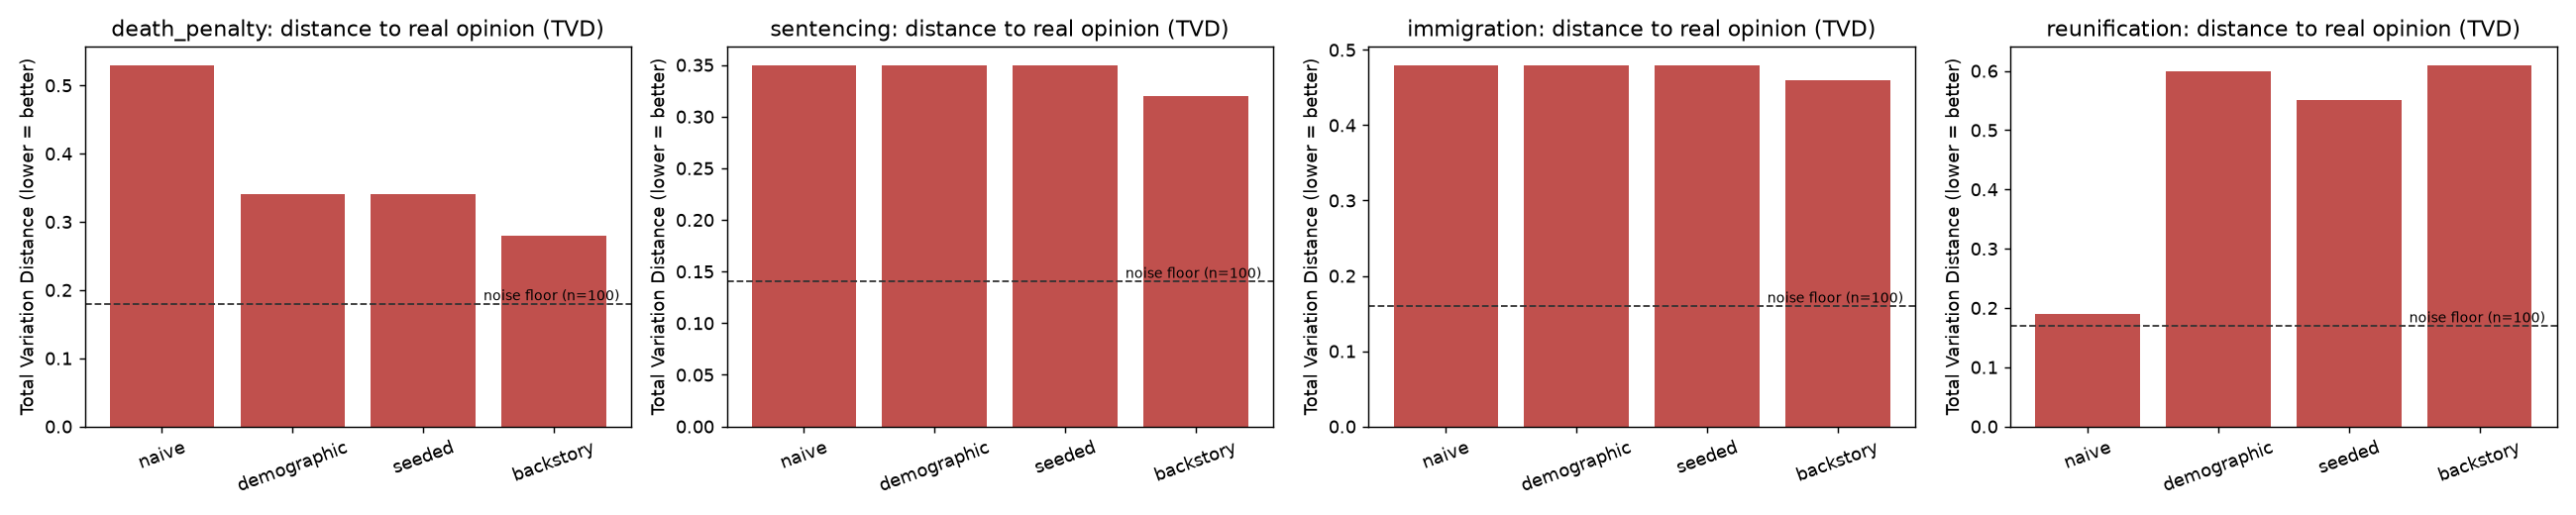
\includegraphics[width=\textwidth]{fig_scorecard.png}
\caption{Distance to real opinion by method, each question against its own noise
floor (dashed). Green bars clear the floor; red bars miss it.}
\label{fig:scorecard}
\end{figure}

Five things came out of the full run, and two of them cut against the ``richer
personas win'' story we expected.

\textbf{1. On the cheap model, the main failure is mode collapse, not being
off-target.} On sentencing and immigration the naive, demographic, and seeded
personas nearly all give the single most common answer: 100\% ``sentences not harsh
enough'' (real: 65\%), 100\% ``reduce immigration'' (real: 52\%). They land the
modal answer and erase everything around it. The variance-ratio metric reads 0.00
where real opinion has spread. This was the failure we most wanted to catch, and it
caught it.

\textbf{2. A stronger model largely fixes the collapse, so it's partly a model
problem rather than the idea's fault.} Re-run on 2.5 Flash, immigration's
demographic method drops from 0.48 (flat collapse) to 0.17, under the noise floor,
and its variance-ratio climbs from 0.00 to 0.70. Sentencing's spread recovers from
0.00 to about 0.6. A lot of ``everything collapses'' was the small model.

\begin{table}[H]
\centering
\begin{tabular}{lcc}
\toprule
Question & Flash-Lite demographic & 2.5 Flash demographic \\
\midrule
Immigration   & 0.48 (var 0.00) & 0.17 (var 0.70) \\
Sentencing    & 0.35 (var 0.00) & 0.30 (var 0.59) \\
Death penalty & 0.34 (var 0.81) & 0.27 (var 0.84) \\
\bottomrule
\end{tabular}
\caption{The same method on a weak and a stronger model. The collapse (variance
0.00) is largely a model-capability effect.}
\end{table}

\textbf{3. The biggest single lever is how you ask, not how rich the persona is.}
Instead of sampling one hard choice per persona, we asked each persona for a
probability across the options, a soft vote, and averaged. On 2.5 Flash this
recovers the real distribution almost exactly: immigration TVD 0.04 (predicted
52/27/13/9 against a real 52/23/17/8), death penalty TVD 0.08. One caveat we hold
to: a smooth average has less variance than 100 hard votes, so it can slip under the
noise floor for mechanical reasons, and we don't claim it beats a real poll. But the
recovery of the actual proportions is real, and large. Asking for the distribution
beats sampling the mode.

\textbf{4. Conditioning cuts both ways, and where the public is genuinely undecided
it hurts.} Reunification splits real Britons three ways (36\% stay, 19\% join, 36\%
no preference). On Flash-Lite the naive method lands closest, 0.19, right at the
floor, because its vagueness keeps the ``no preference'' third. Add demographics or a
backstory and personas swing to 96--97\% ``stay in the UK'', which drives TVD to
0.60 by inventing a certainty that isn't there. A richer identity makes a persona
pick a side, which is right when the public has picked one and wrong when it hasn't.
(On 2.5 Flash the effect is milder, demographic 0.24 against naive 0.25, because the
stronger model holds the ambivalence better.)

\textbf{5. The persona ladder isn't a straight climb.} On 2.5 Flash death penalty,
demographic (0.27) beats backstory (0.34), because the backstory over-commits to
``strongly support''. And the naive baseline collapses in a model-specific
direction: toward ``tend to support'' on Flash-Lite, toward ``don't know'' and
``oppose'' on 2.5 Flash. The richest method doesn't always win.

The subgroup panels (Figure~\ref{fig:subgroups} shows one) carry the same story a
level down: they test whether simulated Leave and Remain voters, or Conservative and
Labour voters, differ the way real ones do, against each subgroup's own wider noise
floor.

\begin{figure}[H]
\centering
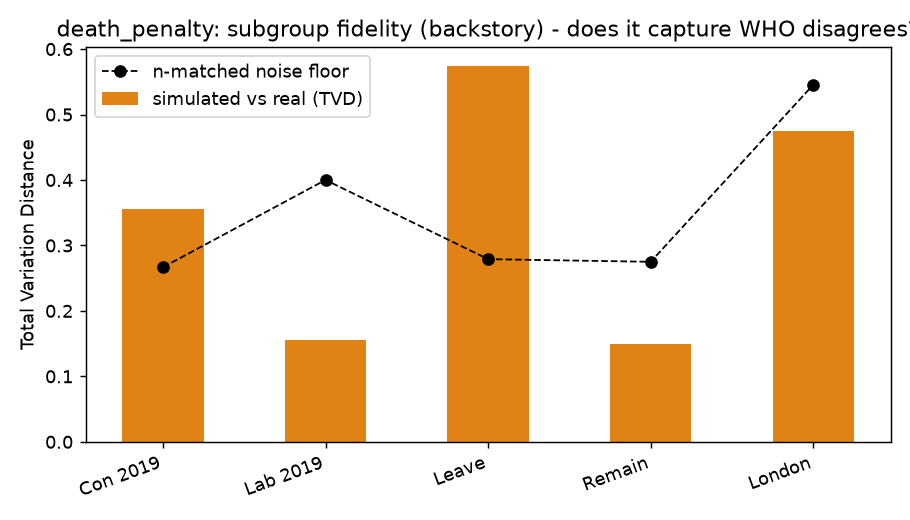
\includegraphics[width=0.82\textwidth]{fig_death_penalty_subgroups.png}
\caption{Subgroup fidelity on the death-penalty question: simulated-vs-real distance
per faction, against each faction's (larger) noise floor.}
\label{fig:subgroups}
\end{figure}

\subsection*{The application question, and whether opinion moves}

With no poll to check against, we put the personas to the minister-liability
question. The group leans support (backstory: about 59\% net support;
Figure~\ref{fig:application}), trustworthy to the degree the validation questions
earned it.

\begin{figure}[H]
\centering
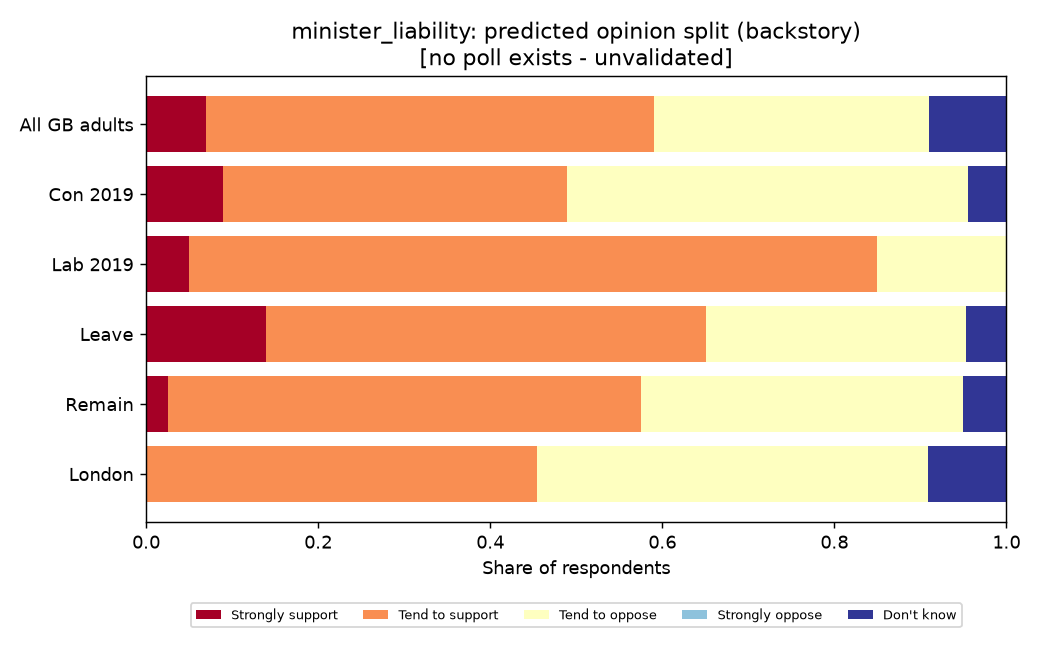
\includegraphics[width=0.9\textwidth]{fig_minister_liability_application.png}
\caption{The un-pollable question: predicted opinion split overall and by faction.}
\label{fig:application}
\end{figure}

Then the part a poll can't cheaply give you: how far opinion moves under different
messaging. We re-ask under two opposing frames plus two controls.

\begin{table}[H]
\centering
\begin{tabular}{lc}
\toprule
Frame & Net support \\
\midrule
Neutral (baseline)              & 71\% \\
Placebo (irrelevant argument)   & 40\% \\
``Accountability''              & 96\% \\
``Chilling effect''             & 9\%  \\
\bottomrule
\end{tabular}
\caption{Net support for minister liability under each frame (backstory personas).}
\end{table}

\begin{figure}[H]
\centering
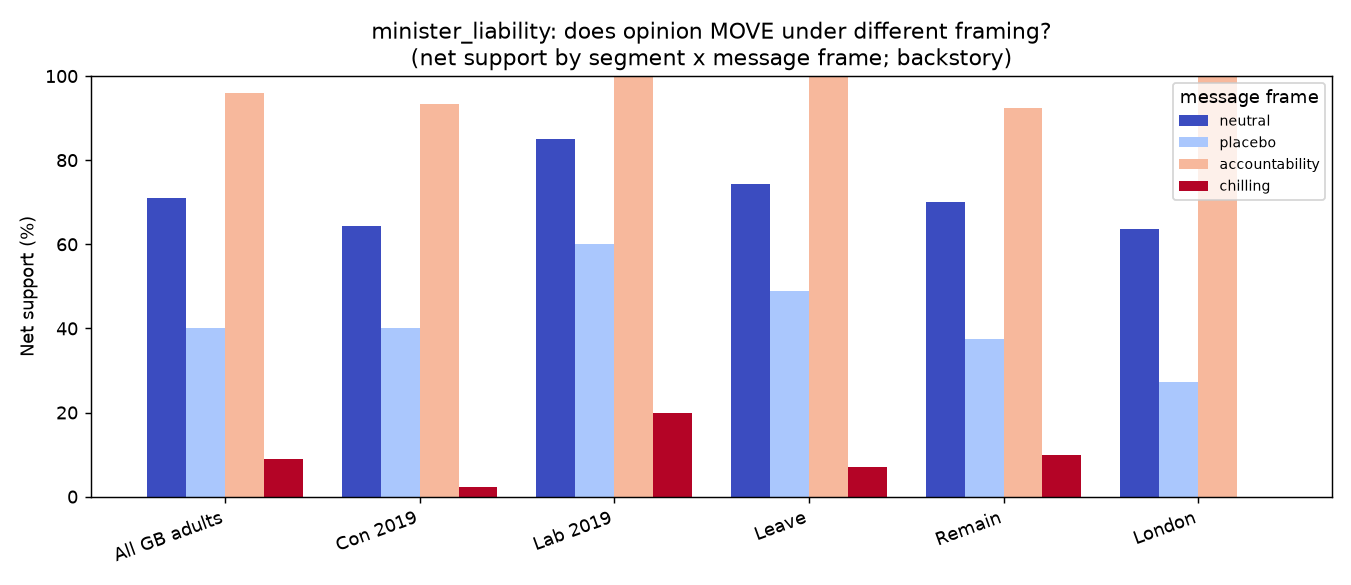
\includegraphics[width=\textwidth]{fig_minister_liability_framing.png}
\caption{Net support by segment under each frame. The gap between a segment's bars
is how far that segment moves between messages.}
\label{fig:framing}
\end{figure}

The swing is enormous, 9\% to 96\%. But the placebo, an argumentative yet irrelevant
preamble about planting street trees, moved support down 31 points on its own. So
roughly a third of any apparent persuasion is just the persona reacting to being
argued at, not to what the argument actually says. Both real frames move well clear
of the placebo in their intended direction, so there's genuine signal in the message
content, but the absolute swings are inflated. Trust the ordering (accountability
lifts, chilling crushes, chilling moves more) rather than the exact points.

Where the run's numbers differ from the shape we assumed going in (collapse
dominating on the cheap model, conditioning hurting on the undecided question, the
ladder not being a straight climb), those differences are the findings. The noise
floor, the variance-ratio, and the placebo are the instruments that surfaced them,
and that's what makes the directional signal worth trusting.

\section*{What this means, and where the limits are}

Where it's reliable: as a fast, cheap, directional read. Which way an audience
leans, which subgroups split, which message has a problem. Run it in an hour,
iterate, and then spend the real survey budget on the finalists.

Where it isn't, yet: as a precise replacement for a poll. The issues we measured or
guarded against:
\begin{itemize}
  \item Variance collapse. Weaker models pile onto the majority answer and throw away minority opinion. We measure it with the variance-ratio rather than hide it, and it eases a lot with a stronger model and with distribution-style asking.
  \item Prompt instability. Answers can move with wording and model version (Bisbee et al.\ 2024). Pin the model and the prompt.
  \item Proxy ground truth. We validate against one poll at one point in time; a different population or date would shift the target.
  \item Seeding data. True per-row seeding (method 3) needs individual-level survey rows, like the British Election Study. Without them that method backs off to demographic sampling, and we say so.
\end{itemize}

\section*{Recommendation}

Use AI personas as a decision accelerator, not a decision maker: a first-pass
instrument to narrow options, surface where audiences split, and pre-test which
message moves which faction, followed by a real poll on the shortlist for anything
consequential.

Two choices mattered more than the persona recipe, and the run is specific about
both:
\begin{itemize}
  \item Use a capable model. The cheap model collapsed to the majority answer; the stronger one recovered real spread and, on two questions, matched the poll within the noise floor. Model capability was a bigger lever than persona richness.
  \item Ask for the distribution, not one vote. Having each persona give a soft probability across the options recovered the real proportions far better than sampling a single choice. It moved fidelity more than anything else we tried.
\end{itemize}

Then keep the guardrails that caught the failures here: run the naive control so the
room can see what conditioning actually buys, report the variance-ratio so a
flattened answer can't pass as a confident one, and put a placebo next to any
message test so suggestibility doesn't get mistaken for persuasion. The message test
is where the leverage is. It turns the simulator from a cheaper poll into something
a poll budget can't buy: a wind-tunnel for messages before you commit to one.

\section*{Appendix, for the technically minded}

\begin{itemize}
  \item \textbf{Metric.} Total Variation Distance (the share of probability mass that would have to move), plus Jensen--Shannon, Wasserstein (for ordinal questions), modal-answer match, and entropy ratio. The framing follows Argyle et al.\ 2023 on algorithmic fidelity.
  \item \textbf{Noise floor.} A bootstrap. Repeatedly draw two n-sized samples from the real distribution and measure their TVD; report the mean and 95th percentile, per subgroup at that subgroup's realised n.
  \item \textbf{Single-select.} Forced through the model's structured-output / enum mode, with option order shuffled per call to cancel position bias. We sample one answer per persona at temperature above zero, one person and one answer, rather than reading an option-probability distribution off the model.
  \item \textbf{Verbalized distribution.} Instead of sampling, each persona returns a probability across the options as structured JSON, which we average. It's scored as an estimate rather than a sample, and judged only on how well it recovers the real proportions.
  \item \textbf{Model and cost.} Provider-agnostic (Gemini or Claude behind one interface). Results here are Gemini Flash-Lite (all five questions) and Gemini 2.5 Flash (the stronger-model cross-check), about \$0.30 in total. Responses are cached on disk, so a run resumes after a rate-limit and re-runs cost nothing.
  \item \textbf{Key references.} Argyle et al.\ 2023 (Out of One, Many); Santurkar et al.\ 2023 (OpinionQA); Park et al.\ 2024 (Generative Agent Simulations of 1,000 People); Moon et al.\ 2024 (Anthology); Bisbee et al.\ 2024 (the instability / flattening critique).
\end{itemize}

\end{document}
